%%%%%%%%%%%%%%%%%%%%%%%%%%%%%%%%%%%%%%%%%%%%%%%%%%%%%%%%%%%%%%%%%%%%%%%%%%%%%%%%%%%%%%%%%%%%%%%%%%%%%%%%%%%%%%%%%%%%%%%%%%%%%%%%%%%%%%%%%%%%%%%%%%%%%%%%%%%%%%%%%%%%%%%%%%%%%%%%%%%%
\chapter{Characterisation and estimation of the Standard Model backgrounds}
\label{sec:BackgroundEstimation}
After the application of the candidate track selection explained in the previous section the background arising from Standard Model processes is dramatically reduced.
However, it still happens sometimes that an electron, muon or tau fails reconstruction.
The underlying mechanism and the methods to estimate the leptonic background will be in detail explained in Section~\ref{sec:LeptiniBkg}.
Furthermore, there is the possibility that a track is reconstructed out of a set of hits which do not origin from only one single particle.
Such tracks are called ``fake tracks''. 
Background tracks arising from the wrong combination of hits will be explained in the following Section~\ref{sec:FakeBkg}

The composition of the background after the candidate track selection is shown in Fig.~\ref{fig:BkgComposition}.
\begin{figure}[!bt]
  \centering 
  \begin{tabular}{c}
    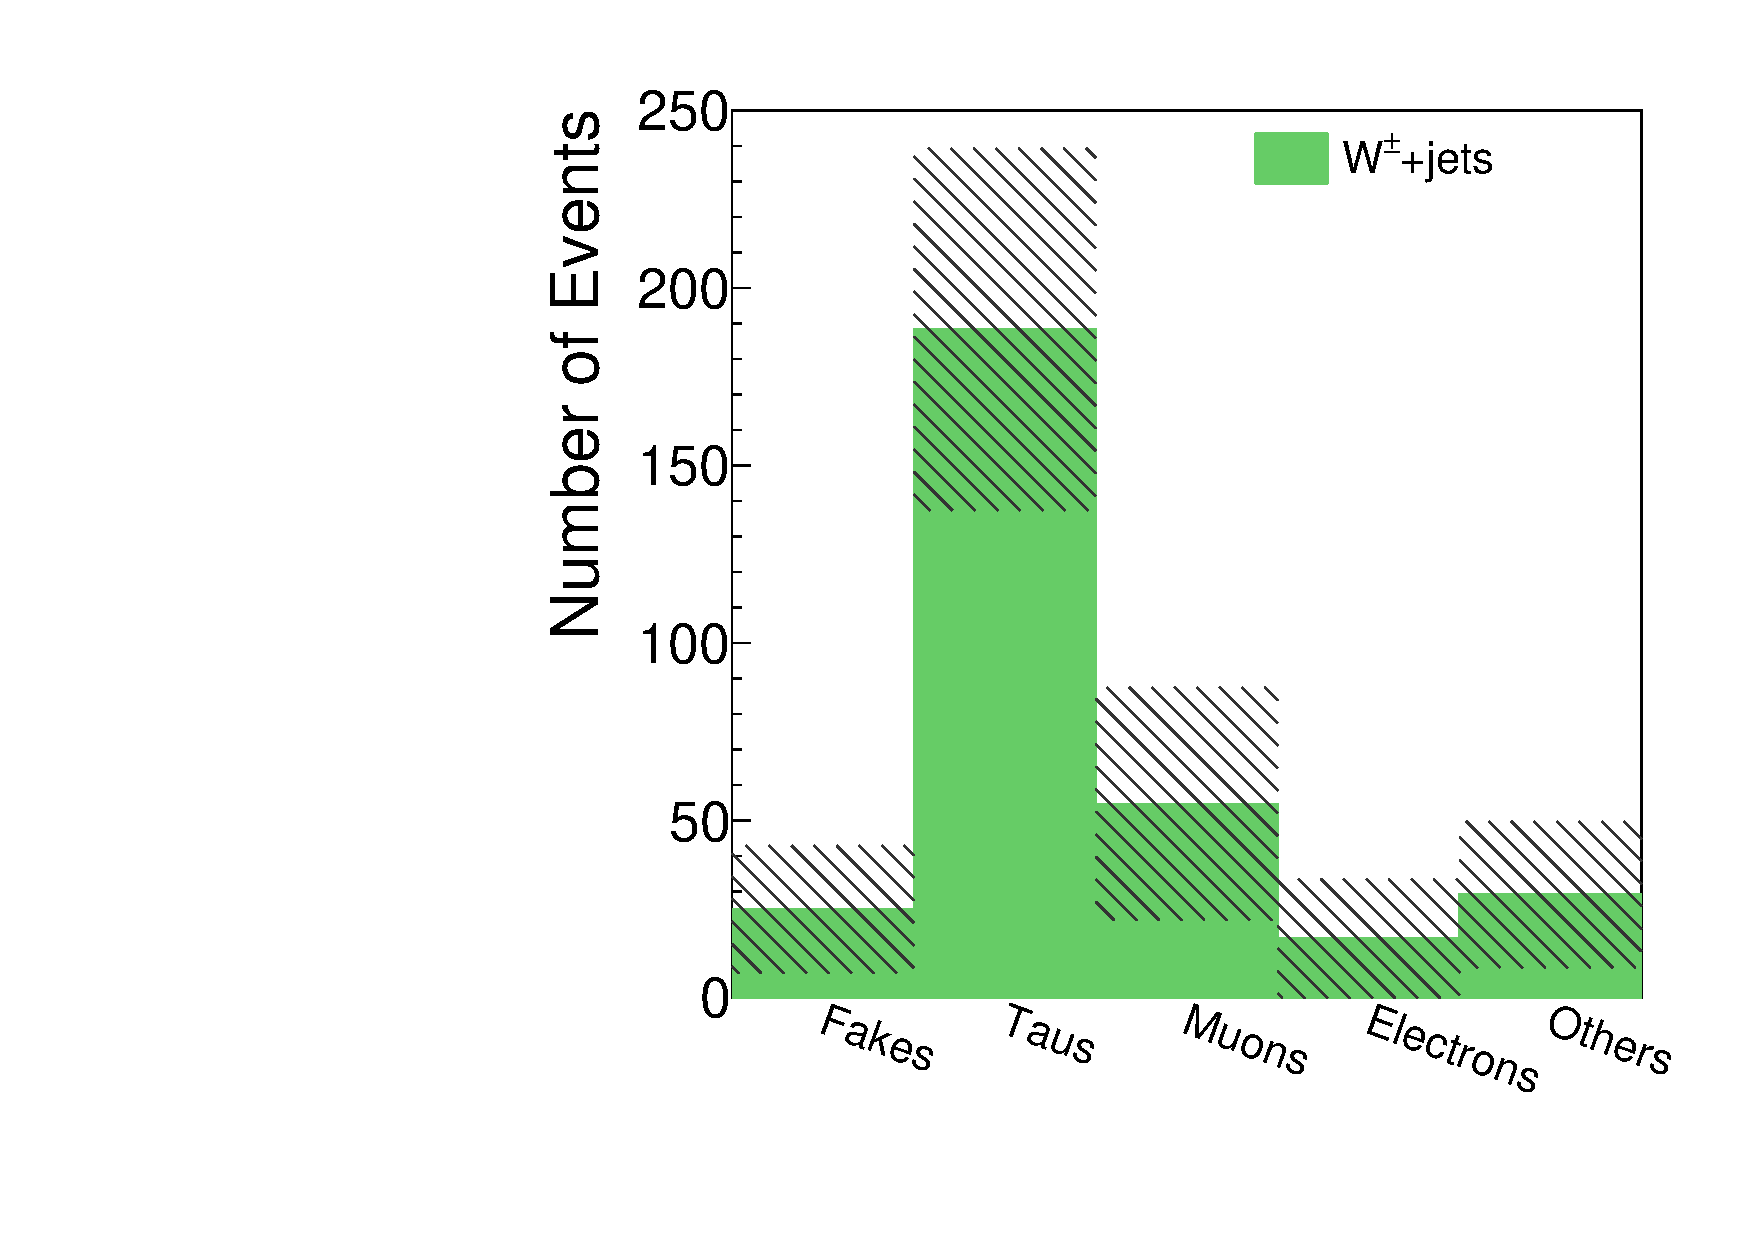
\includegraphics[width=0.49\textwidth]{figures/analysis/htrackgenParticleSmallRange_lin_chiTracksfullSelectionTrigger.pdf}
    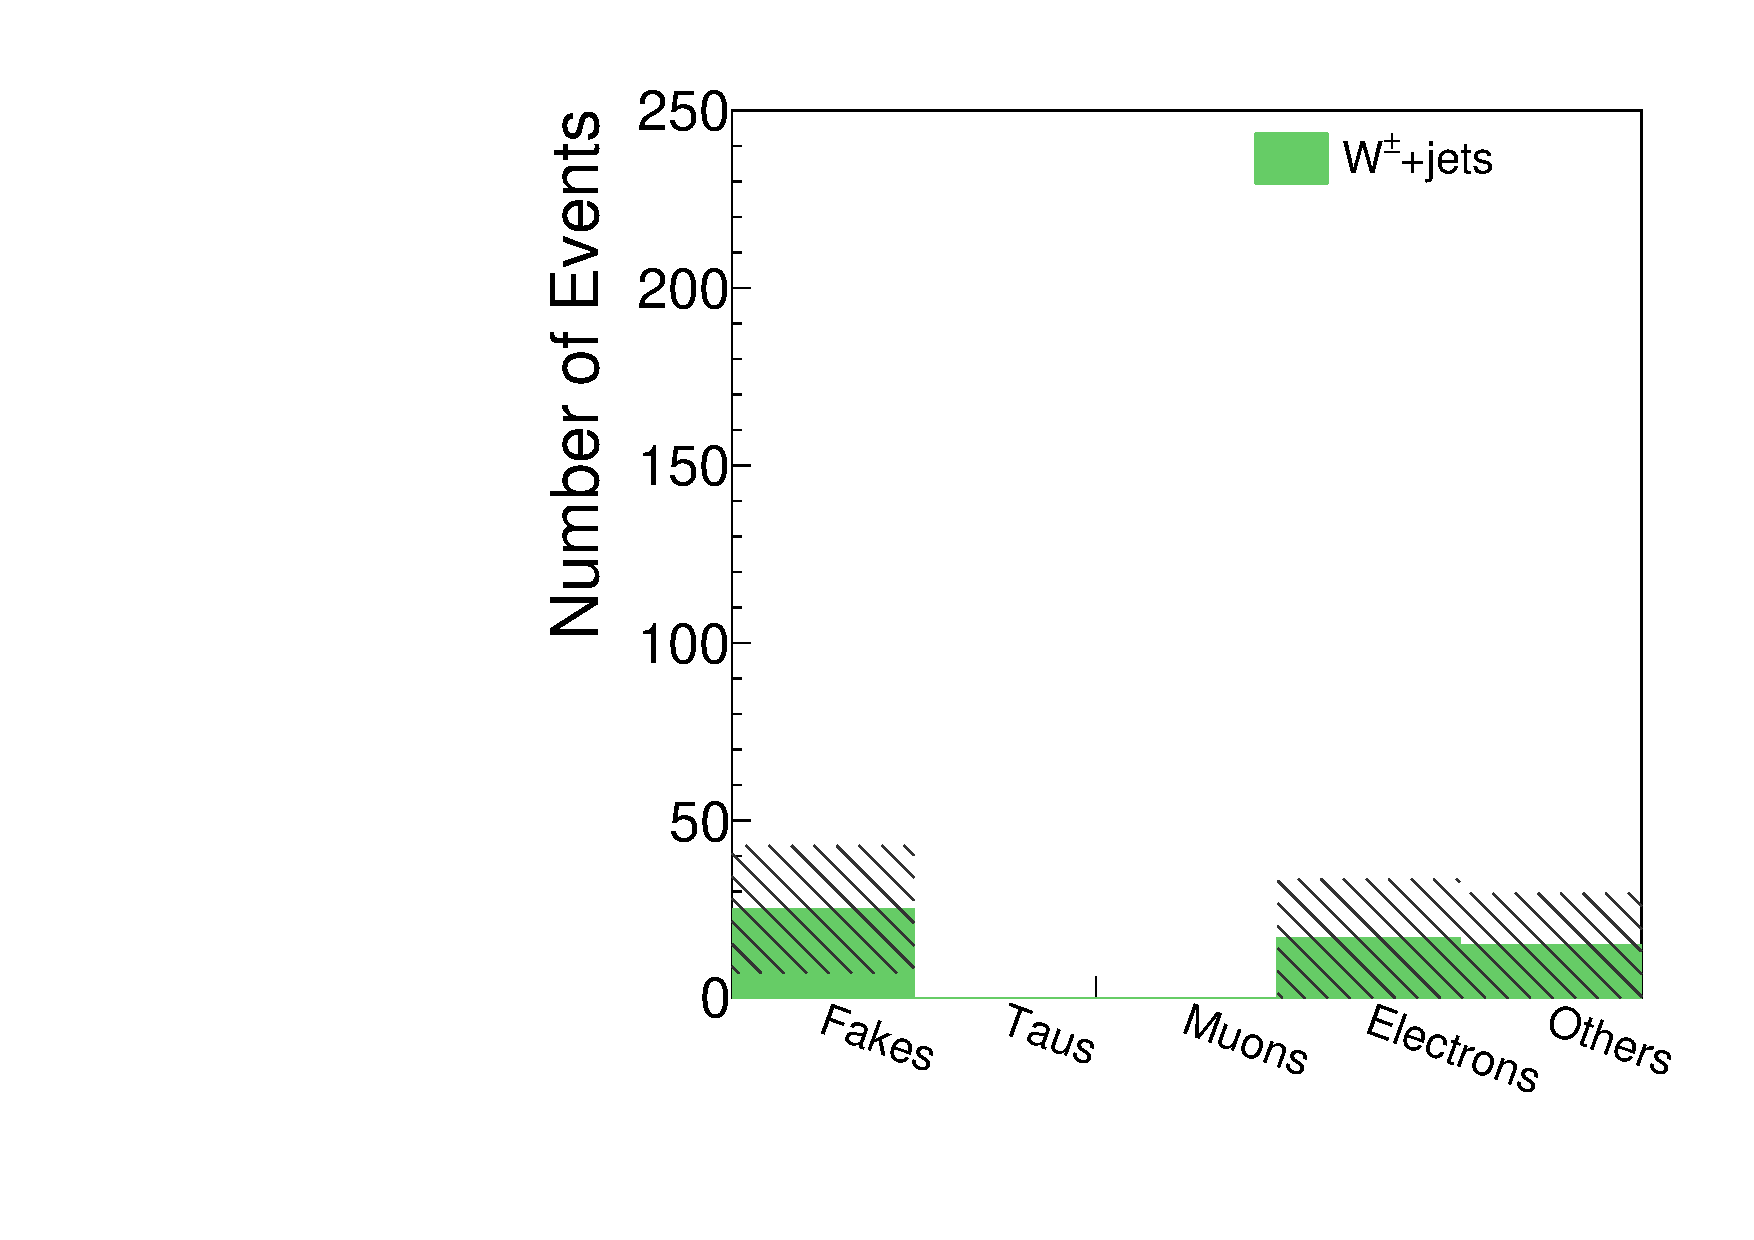
\includegraphics[width=0.49\textwidth]{figures/analysis/htrackgenParticleSmallRange_lin_chiTracksfullSelectionPlusIasTrigger.pdf}
  \end{tabular}
  \caption{Background composition after the full candidate track selection (left) and after the full candidate track selection plus an additional selection cut of \mbox{$\ias>0.05$} (right). 
           The statistical uncertainty is depicted by the hashed grey area.
           Given the limited size of the simulated \WJets dataset, the uncertainty of the composition is accordingly large.}
  \label{fig:BkgComposition}
\end{figure}
This composition can change significantly when imposing further selection cuts on \pt and \ias.
This, however, will be addressed during the optimisation procedure.
To get a feeling how the composition of the background is affected by further cuts on one of the main variables, 
the background composition is also shown with the candidate track selection plus an additional \ias cut of 0.05.
It can be seen that the fake background is less reduced by an additional selection cut on \ias.
This gains even more in importance when considering all sources of fake tracks.
The fake background is not only present in \WJets events but essentially in all Standard Model processes.\\

Still, also the leptonic background can be important.
Unfortunately, because of the limited size of the simulated \WJets dataset, it is not possible to study the leptonic contribution to the background with simulated events.
Furthermore, when the simulation of the operativeness of every single detector module is not fully correct, the simulation could highly underestimate the leptonic background.\\

Therefore, a data-based approach is needed for either of the two background sources: the fake and the leptonic background.
%%%%%%%%%%%%%%%%%%%%%%%%%%%%%%%%%%%%%%%%%%%%%%%%%%%%%%%%%%%%%%%%%%%%%%%%%%%%%%%%%%%%%%%%%%%%%%%%%%%%%%%%%%%%%%%%%%%%%%%%%%%%%%%%%%%%%%%%%%%%%%%%%%%%%%%%%%%%%%%%%%%%%%%%%%%%%%%%%%%%
%%%%%%%%%%%%%%%%%%%%%%%%%%%%%%%%%%%%%%%%%%%%%%%%%%%%%%%%%%%%%%%%%%%%%%%%%%%%%%%%%%%%%%%%%%%%%%%%%%%%%%%%%%%%%%%%%%%%%%%%%%%%%%%%%%%%%%%%%%%%%%%%%%%%%%%%%%%%%%%%%%%%%%%%%%%%%%%%%%%%
\section{Fake background}
\label{sec:FakeBkg}
Fake tracks are tracks which are not reconstructed out of the trajectory of one single particle.
The rate with which this wrong reconstruction occurs is of course highly restrained by the quality cuts on $\chi^2$ and the vertex compatibility of the track reconstruction algorithm.
Details on the reconstruction algorithm at CMS can be found in Section~\ref{FIXME}.
The fake rate is strongly correlated to the number of hits in the tracker system. 
This can be seen in Fig~\ref{fig:NValidFakes}, where the distribution in the number of hits of fakes is depicted.
\begin{figure}[!bt]
  \centering 
  \begin{tabular}{c}
    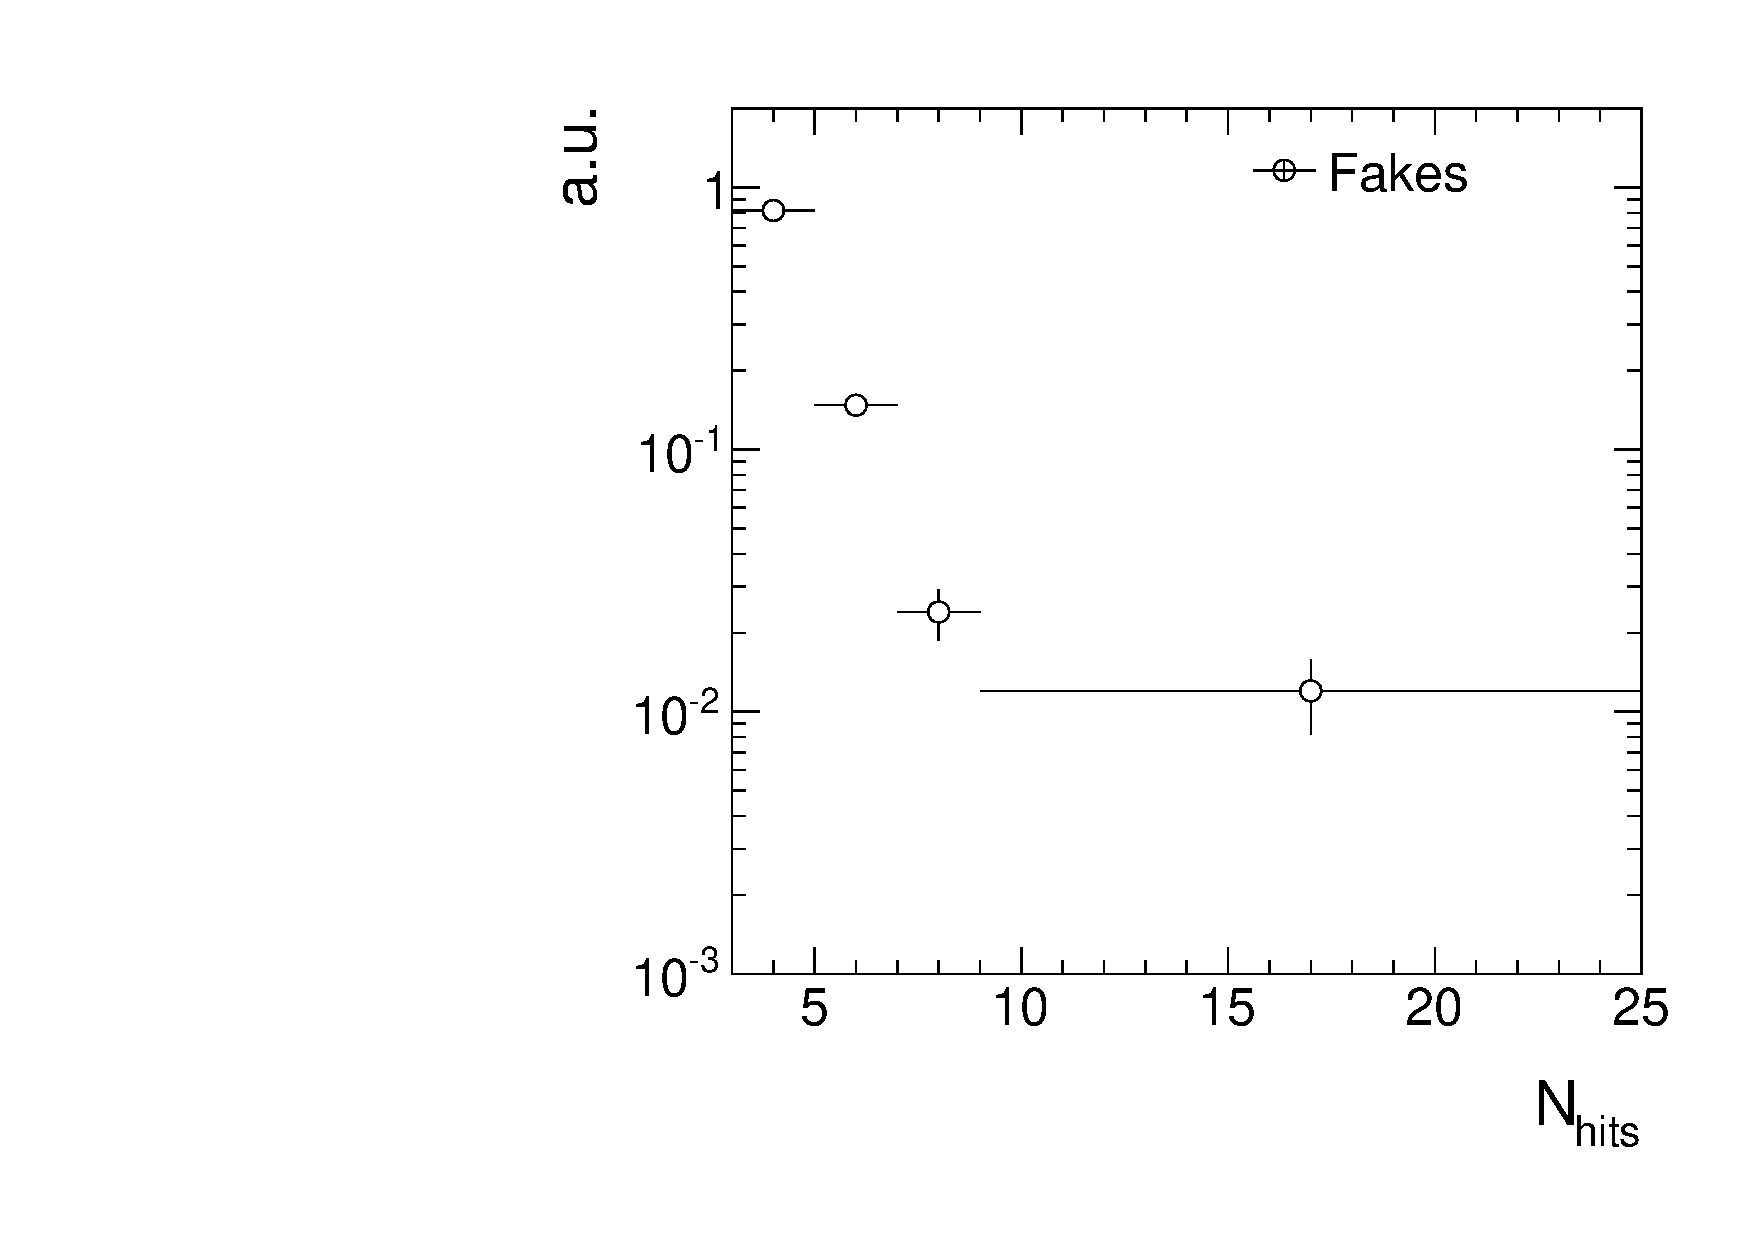
\includegraphics[width=0.49\textwidth]{figures/analysis/NValidForFakes_chiTracksfullSelectionNoQCDCutsNoTrigger_PtGt15GeV.pdf}
  \end{tabular}
  \caption{bla bla}
  \label{fig:NValidFakes}
\end{figure}
In simulation, fake tracks are defined as tracks which cannot be matched to a generator-level particle within a distance of $\Delta R < 0.01$.
This can happen due to pile up and maybe there are other reasons.

Fakes are efficiently suppressed by the vertex compatibilyt selection cuts and the no missing middle and inner hits requirement.
Unfortunately, when they pass these criteria, thay also pass the \ecalo cut with high efficiency because they do not origin from a real particle.\\

In this analysis, the fake background estimation is split into two seperate parts.
First an estimation of the fake background is done which is incluseveliy in \ias.
As a second step, the ias distribution is taken from a fake enriched control region.

The inclusive background estimation follows closely the background estimation method done in \cite{blabla}.
For this a dysample with blabla
is taken.

\begin{itemize}
\item Show plot with fake rate in different samples
\item Show dependency of fakes for the number of hits
\item Show ias plot for fakes
\item Explain background estimation method
\end{itemize}
%%%%%%%%%%%%%%%%%%%%%%%%%%%%%%%%%%%%%%%%%%%%%%%%%%%%%%%%%%%%%%%%%%%%%%%%%%%%%%%%%%%%%%%%%%%%%%%%%%%%%%%%%%%%%%%%%%%%%%%%%%%%%%%%%%%%%%%%%%%%%%%%%%%%%%%%%%%%%%%%%%%%%%%%%%%%%%%%%%%%

\section{Leptonic background}
\label{sec:LeptonicBkg}

The leptonic background of the presented search is caused by non-reconstructed leptons which undergo hence the lepton veto selection.
However, at least non-reconstructed electrons or taus should in principle deposit enough energy in the calorimeters such that they can still be vetoed by the calorimeter isolation requirement.
As muons don't deposit much energy in the calorimeters, this reason does not hold for them.
In the following, the sources of the three different leptonic backgrounds shall be characterised.

\subsection*{Electrons}
To avoid the background source from unreconstructed electrons, all tracks pointing to a dead or noisy ECAL cells are vetoed, as described in the previous section.
By this selection, almost all electrons are efficiently rejected.
In the simulated \WJets sample only one simulated event remains which pass all candidate track selection criteria and where the candidate track can be matched to a generator-level electron.
This event is visualised in Fig~\ref{fig:LostElectron}. 
\begin{figure}[!tb]
  \centering 
  \begin{tabular}{c}
    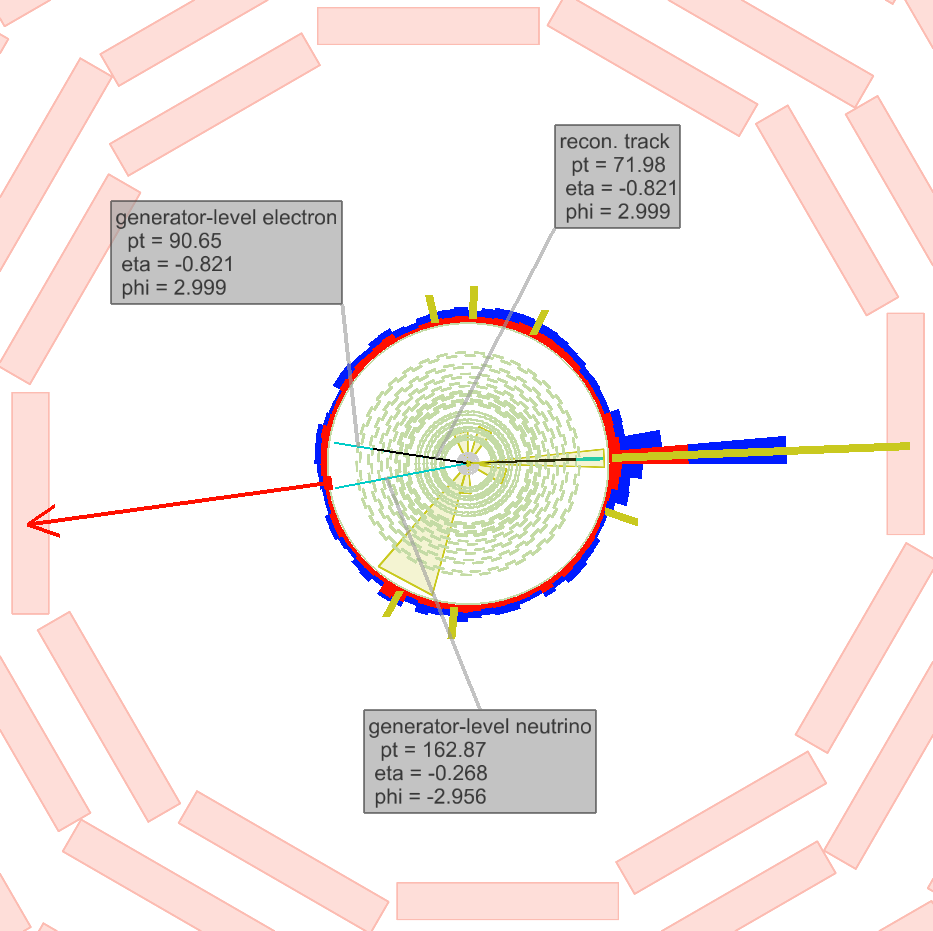
\includegraphics[width=0.49\textwidth]{figures/analysis/Electron_lumi_279317_event_111637553.png}
  \end{tabular}
  \caption{Visualisation of an $W\rightarrow e\nu_e$ event contributing to the SM background. 
           In light blue the generator-level particles $e$ and $\nu_e$ of the $W$ decay are shown. 
           The $\nu_e$, only weakly interacting does not show any signature in the detector, whereas the electron ($\pt\simeq 90\gev$) leaves a track (black line) with \mbox{$\pt\simeq 70\gev$} in the tracker. 
           No ECAL energy deposits in the direction of the electron are visible. 
           This is caused by the fact that the corresponding ECAL energy deposits were not read out in this event.
           An ISR jet ($\pt\simeq 230\gev$) causes the \met (read arrow) in the event. }
  \label{fig:LostElectron}
\end{figure}
In this event no energy deposits in the ECAL are read out, which suggests, that this ECAL tower was neither working properly in 2012.
Additionally, electrons can do bremsstrahlung which can change the direction of the electron significantly.
Thus, the energy deposits in the ECAL can possibly not be matched to the original electron.


\subsection*{Taus}
The tau background is contributing through the hadronic decay of a tau lepton to one charged pion $\tau\rightarrow\pi^{\pm}\nu$.
Unreconstructed taus are typically low energetic and can therefore bypass the calorimeter isolation criterion.
Because of nuclear interactions in the tracker, they can result in short reconstructed tracks which can easily be highly mismeasured in \pt.
Thus, pions can also contribute even when imposing a tighter selection in the transverse momentum.
Such an event is shown in Fig.~\ref{fig:LostTau}.
\begin{figure}[!tb]
  \centering 
  \begin{tabular}{c}
    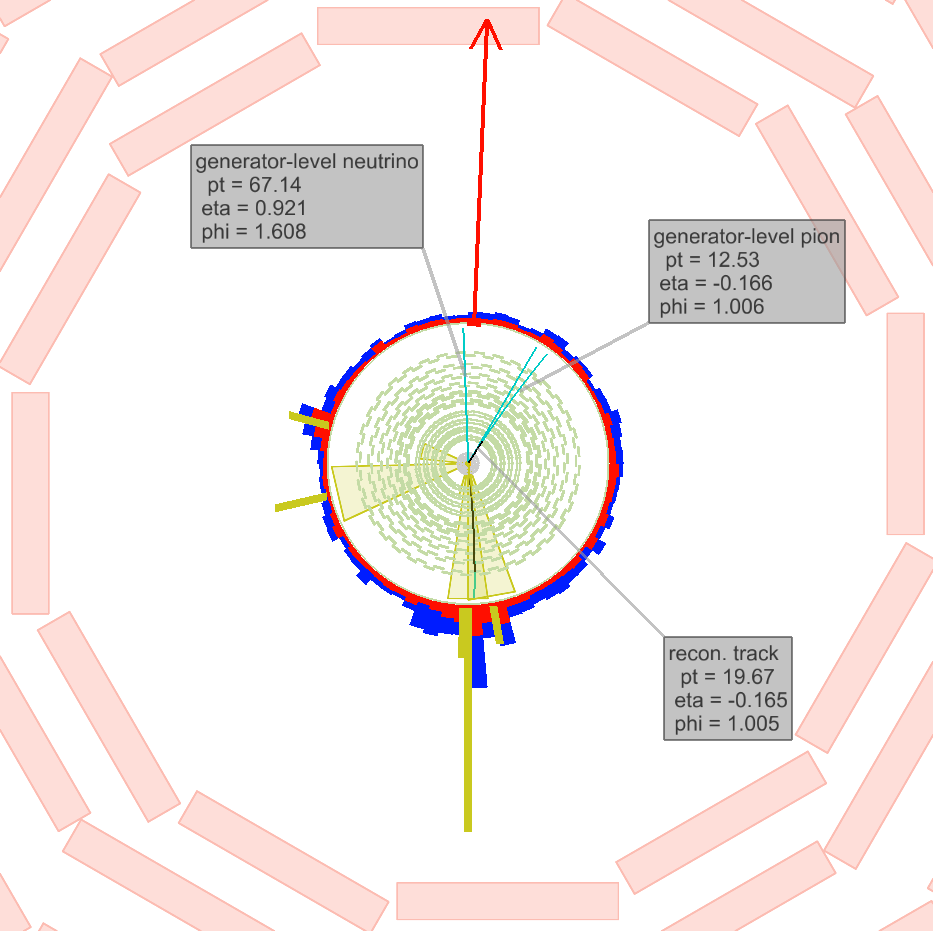
\includegraphics[width=0.49\textwidth]{figures/analysis/LostTau_Lumi_60133_Event_24033837.png}
  \end{tabular}
  \caption{Visualisation of a $W^{+}\rightarrow \tau^{+}\nu_{\tau} \rightarrow \pi^{+} \nu_{\tau}$ event contributing to the SM background. 
           In light blue the generator-level particles $\pi^{+}$ and $\nu_{\tau}$ are shown.
           The reconstructed track (black line) is very short because the pion interacts with the tracker material via the strong force.}
  \label{fig:LostTau}
\end{figure}

\subsection*{Muons}
Muons can fail reconstruction when they are pointing towards a bad cathode strip chamber.
This is taken into account in the candidate track selection.
However, some of the muons still fail reconstruction when they fall within the gap between stations 0 and 1 of the DT system at $\eta=0.25$.
The muon reconstruction efficiency drops from around 99\% to a value of around 94\% as shown in~\ref{jessicathesis}. 
This possibility is illustrated in a simulated event shown in Fig~\ref{fig:LostMuon}.
\begin{figure}[!tb]
  \centering 
  \begin{tabular}{c}
    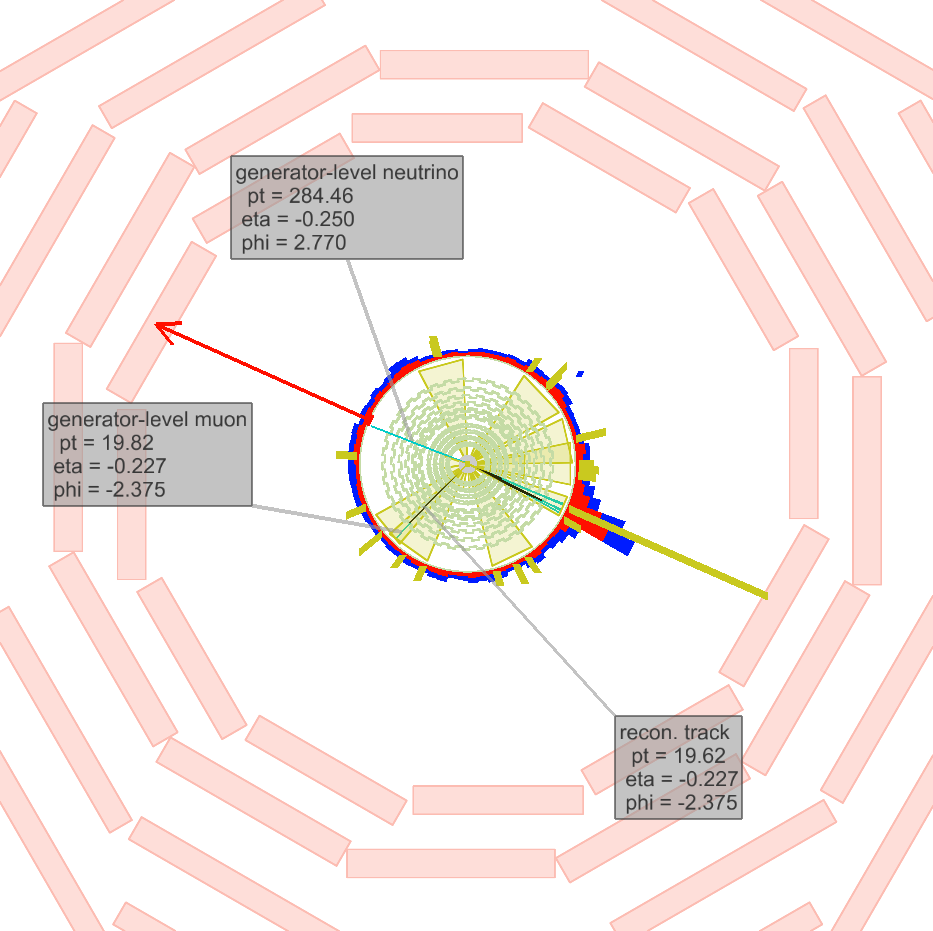
\includegraphics[width=0.49\textwidth]{figures/analysis/LostMuon_Lumi_357583_Event_142918834.png}
  \end{tabular}
  \caption{Visualisation of an $W\rightarrow \mu\nu_{\mu}$ event contributing to the SM background. 
           In light blue the generator-level particles $\mu$ and $\nu_{\mu}$ of the $W$ decay are shown. }
  \label{fig:LostMuon}
\end{figure}
In~\ref{jessicastheisi} events are rejected when the track is pointing in a region of $0.15<|\eta|<0.35$.
In this search, this cut was omitted to maximise signal acceptance. 
Due to the additional selection in \ias, muons can easily be efficiently suppressed.
E.g. in the event example shown in Fig~\ref{fig:LostMuon}, the muon has an \ias value of about 0.02.\\


In general, all leptons are rather minimal ionising, especially muons and pions.
Electrons can more easily interact with the shell electrons of the tracker material, but still the \ias spectrum is quickly decreasing compared to the signal.
To have the possibility to make an optimisation in the two main discriminating variables \pt and \ias, the background estimation methods are designed to work for all different \pt and \ias selection cuts.
A comparison of the \ias distribution for all four different background sources is shown in Fig~\ref{fig:IasDist}.
\begin{figure}[!tb]
  \centering 
  \begin{tabular}{c}
    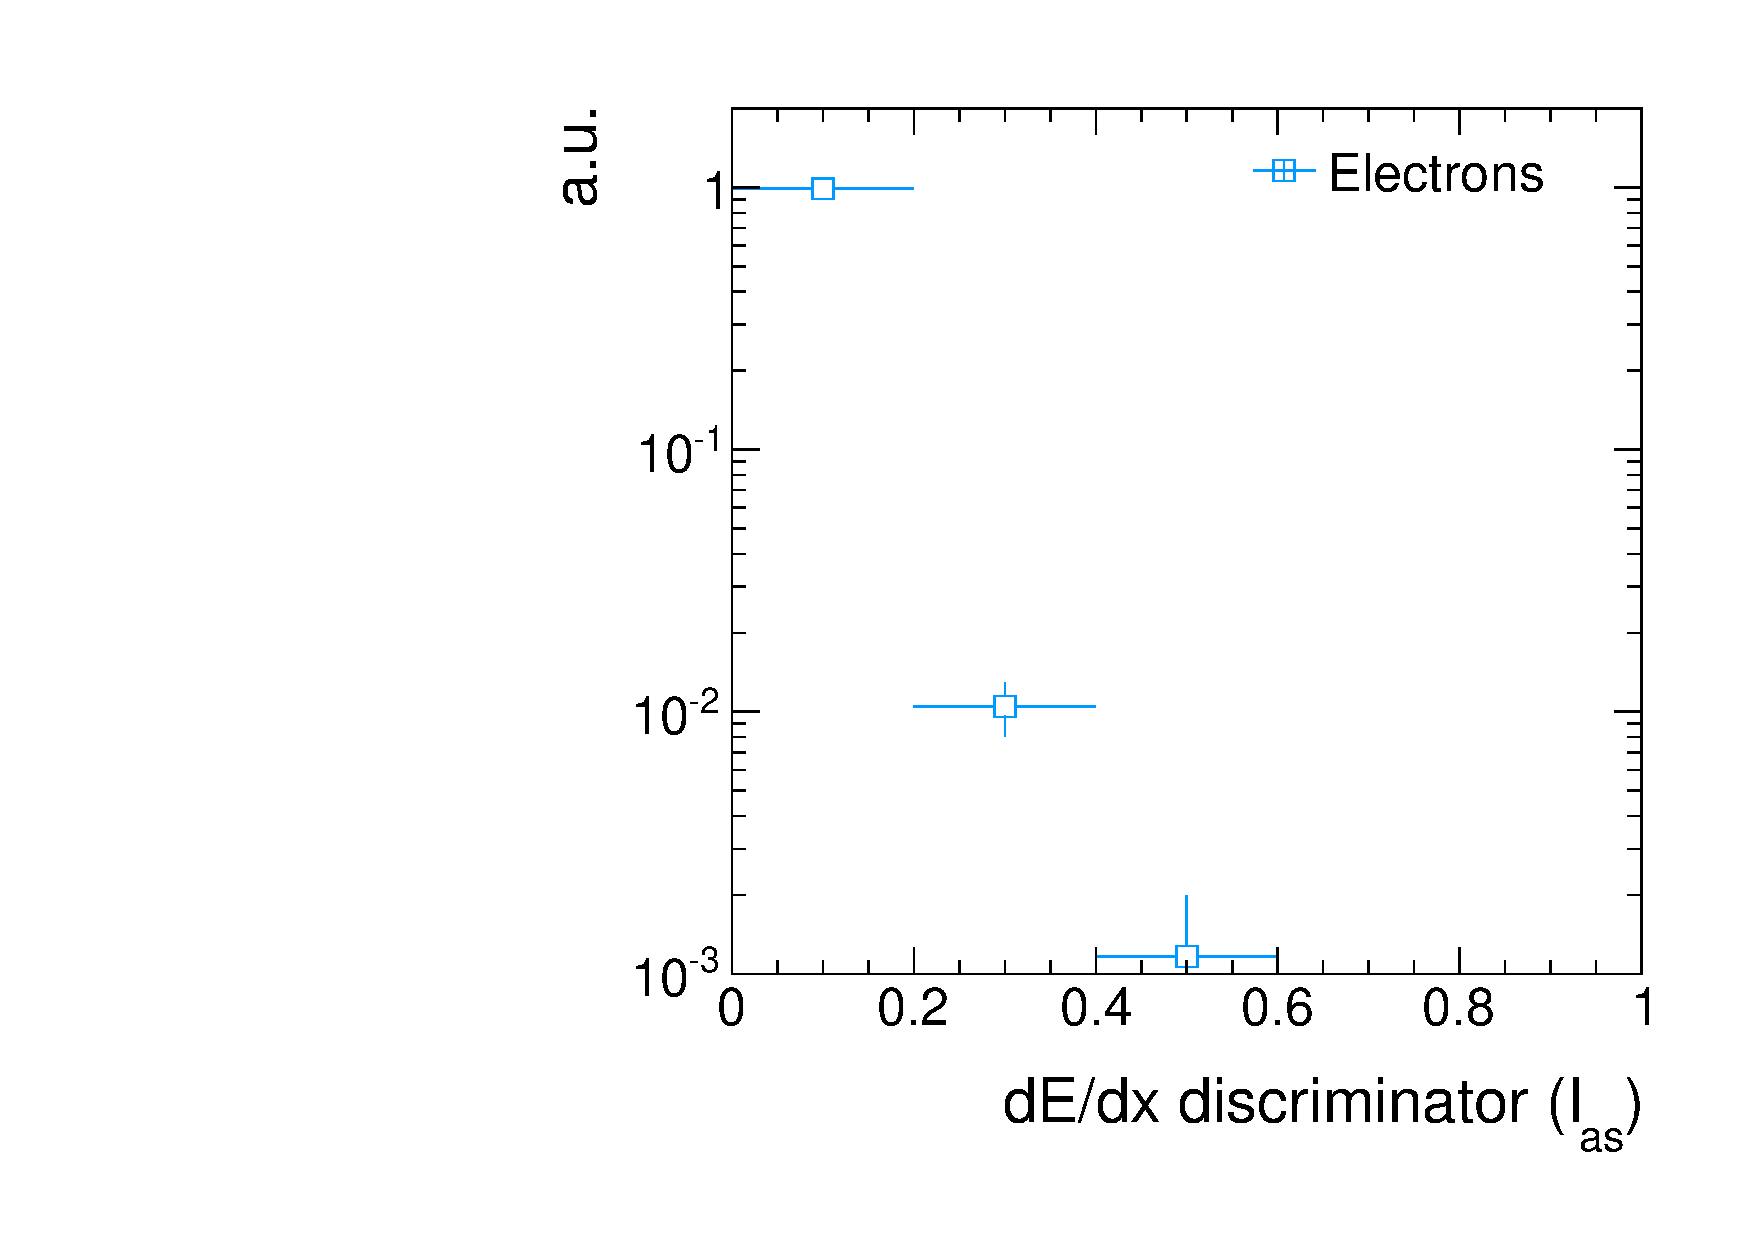
\includegraphics[width=0.33\textwidth]{figures/analysis/IasDistributionForElecs.pdf}
    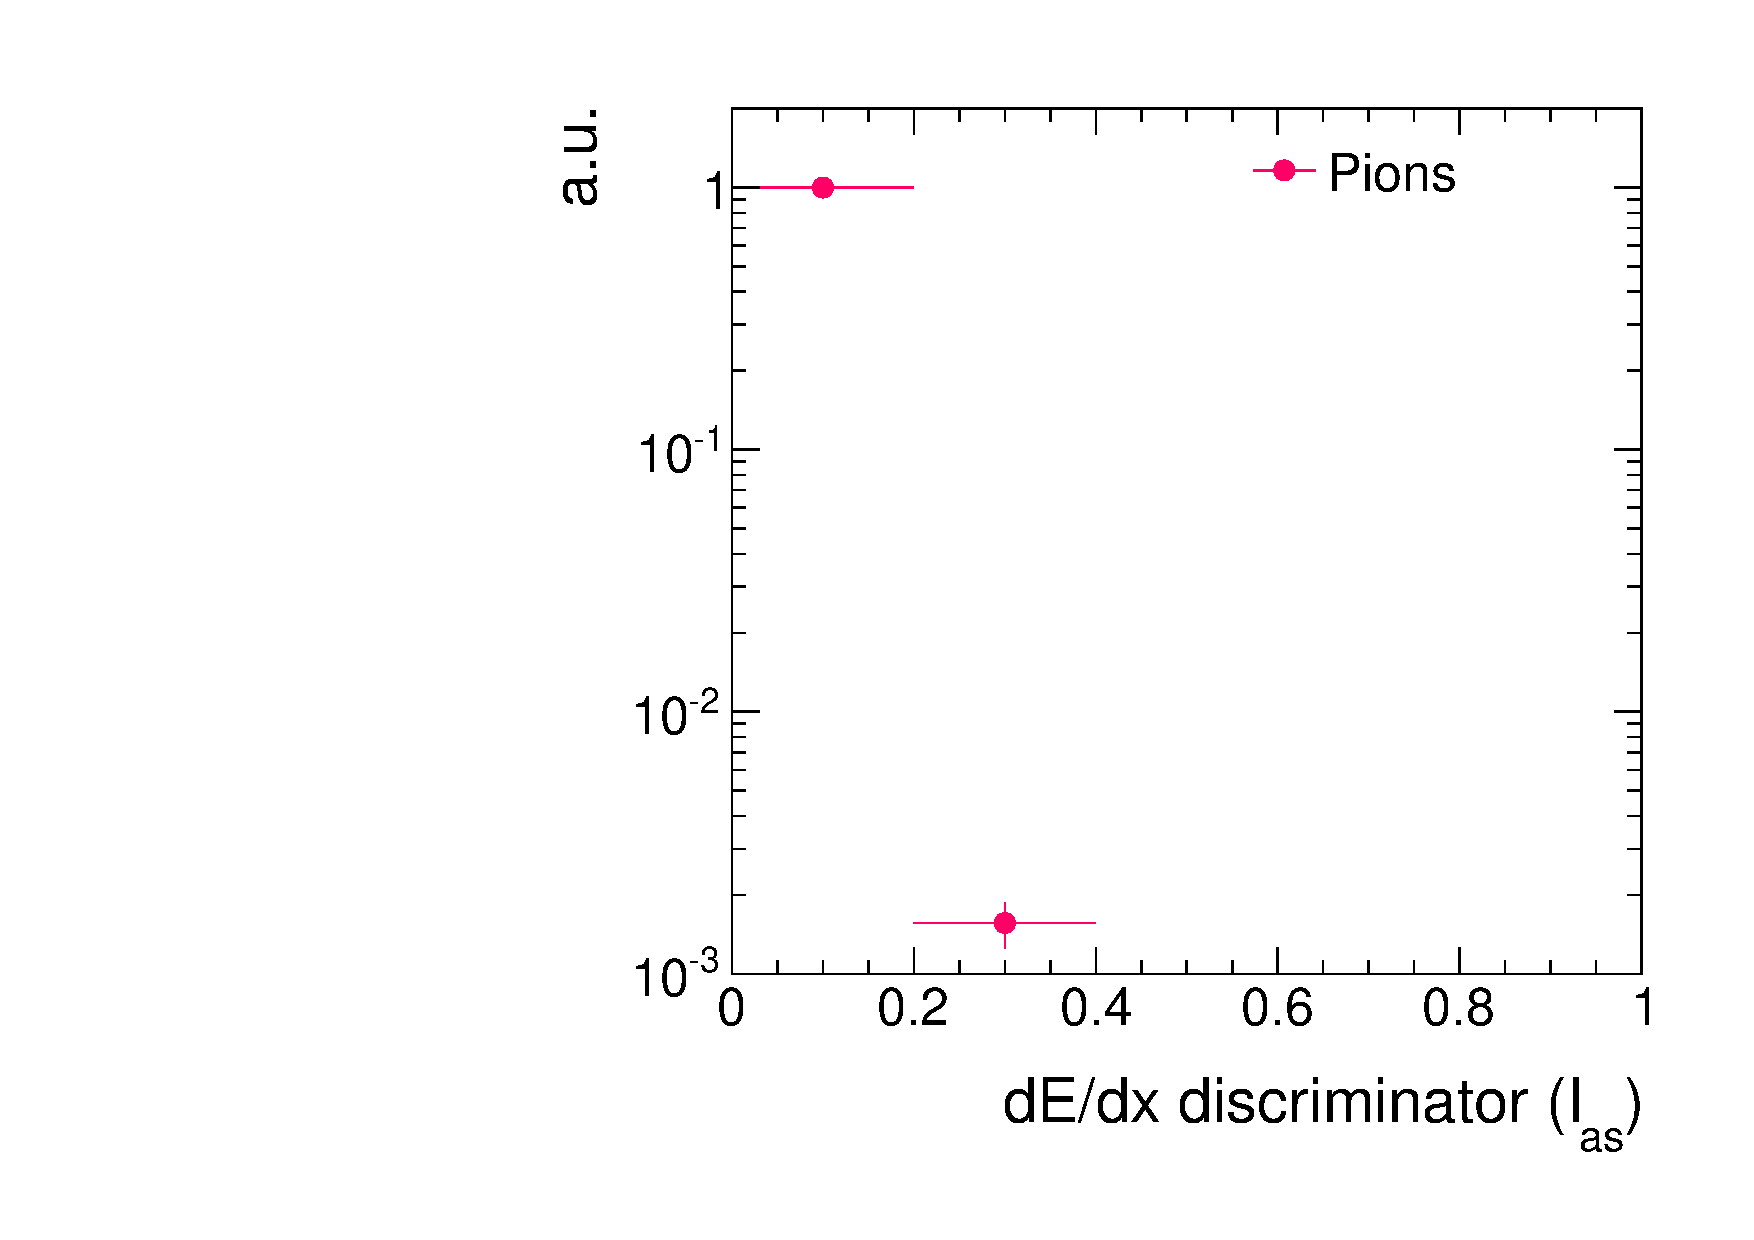
\includegraphics[width=0.33\textwidth]{figures/analysis/IasDistributionForPions.pdf}
    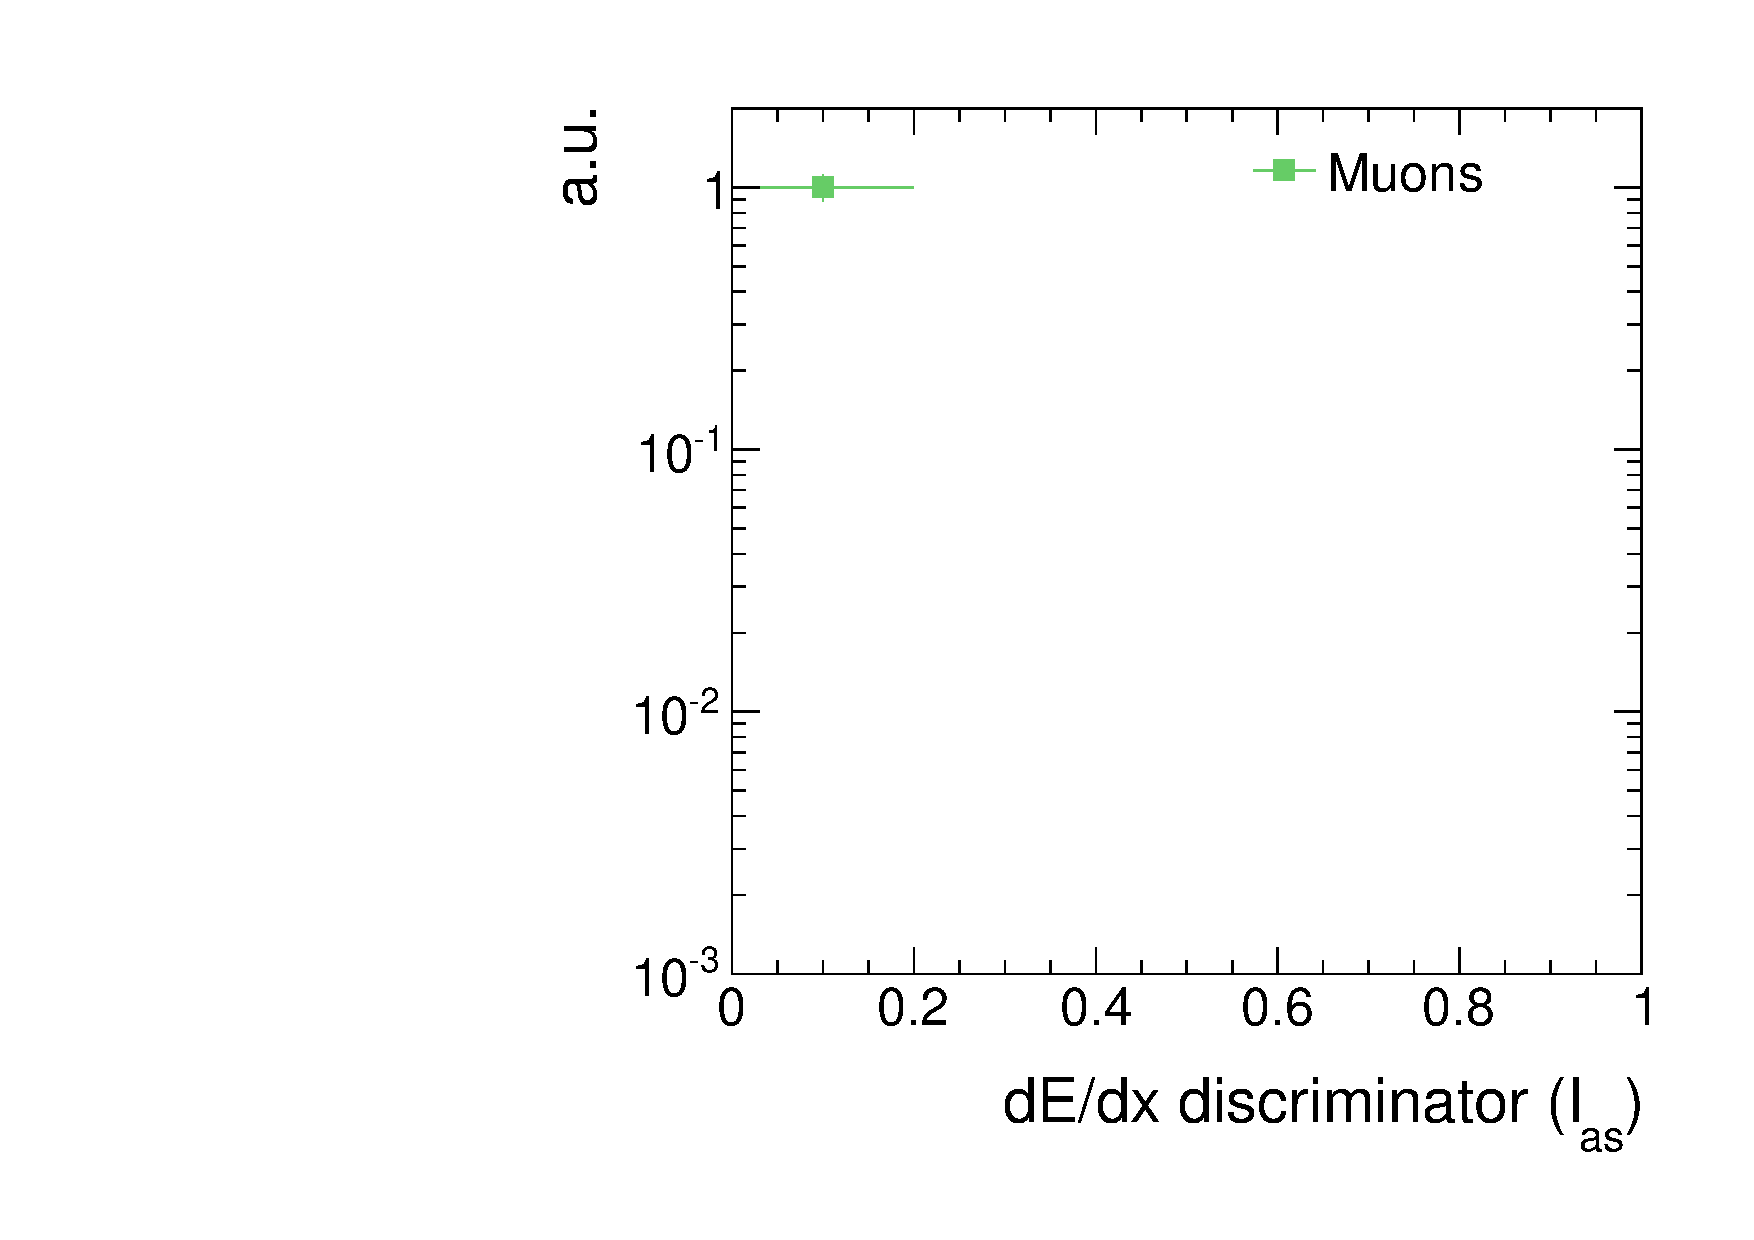
\includegraphics[width=0.33\textwidth]{figures/analysis/IasDistributionForMuons.pdf}
  \end{tabular}
  \caption{Normalised \ias distribution for electrons (left), pions (middle) and muons (right). 
           For all leptons the \ias distribution is rapidly falling.}
  \label{fig:IasDist}
\end{figure}

\section{Systematic uncertainties}
\label{sec:SysUncertaintiesBkg}


\begin{itemize}
\item Background consist of particles which make high energy deposits and are high pt
\item In general: Low background search
\end{itemize}
%%%%%%%%%%%%%%%%%%%%%%%%%%%%%%%%%%%%%%%%%%%%%%%%%%%%%%%%%%%%%%%%%%%%%%%%%%%%%%%%%%%%%%%%%%%%%%%%%%%%%%%%%%%%%%%%%%%%%%%%%%%%%%%%%%%%%%%%%%%%%%%%%%%%%%%%%%%%%%%%%%%%%%%%%%%%%%%%%%%%
%%%%%%%%%%%%%%%%%%%%%%%%%%%%%%%%%%%%%%%%%%%%%%%%%%%%%%%%%%%%%%%%%%%%%%%%%%%%%%%%%%%%%%%%%%%%%%%%%%%%%%%%%%%%%%%%%%%%%%%%%%%%%%%%%%%%%%%%%%%%%%%%%%%%%%%%%%%%%%%%%%%%%%%%%%%%%%%%%%%%
\chapter{Optimisation of search sensitivity}
\label{sec:Optimization}
\begin{itemize}
\item Show plots
\item show table
\item Include NlostOuter here, too
\end{itemize}


%%%%%%%%%%%%%%%%%%%%%%%%%%%%%%%%%%%%%%%%%%%%%%%%%%%%%%%%%%%%%%%%%%%%%%%%%%%%%%%%%%%%%%%%%%%%%%%%%%%%%%%%%%%%%%%%%%%%%%%%%%%%%%%%%%%%%%%%%%%%%%%%%%%%%%%%%%%%%%%%%%%%%%%%%%%%%%%%%%%%
\chapter{Results}
\label{sec:Results}
\begin{itemize}
\item Data cutflowtable
\item Tables with results
\item One plot (4 bins: Prediction and data)
\end{itemize}

%%%%%%%%%%%%%%%%%%%%%%%%%%%%%%%%%%%%%%%%%%%%%%%%%%%%%%%%%%%%%%%%%%%%%%%%%%%%%%%%%%%%%%%%%%%%%%%%%%%%%%%%%%%%%%%%%%%%%%%%%%%%%%%%%%%%%%%%%%%%%%%%%%%%%%%%%%%%%%%%%%%%%%%%%%%%%%%%%%%%
\chapter{Interpretation}
\label{sec:Interpretation}
\section{Systematic uncertainties of simulated signal samples}
\section{Statistical Methods/ Limit setting}
\section{Exclusion limits}
\begin{itemize}
\item 1-d limits
\item 2-d limits
\end{itemize}

